\documentclass{article}

\newenvironment{proof}{\par \noindent {\bf Proof:}}{\begin{flushright}$\Box$\end{flushright}\par \noindent}
\newtheorem{theorem}{\bf Theorem}
\newtheorem{definition}[theorem]{\bf Definition}
\newtheorem{lemma}{\bf Lemma}
\newtheorem{corollary}[theorem]{\bf Corollary}
\newcommand{\pari}{\hspace{\parindent}}

\usepackage{amsmath}
\usepackage{latexsym}
\usepackage{amssymb}
\usepackage{listings}
\usepackage{tikz}


\begin{document}

\title{Aspects of Domain Theory: a Formal Study of Semivaluations}

\author{Teng Yu}


\maketitle



\begin{abstract}
{\it Domain Theory provides the formal foundation for Denotational Semantics of Programming Languages. Quantitative Domain Theory is concerned with metric basic approaches to Domain Theory, with applications to real number computation and complexity analysis. One important concept in this area is the notion of a semivalution. We study this notion, and investigate novel results in this area. 
}
\end{abstract}

\newpage

\tableofcontents

\newpage

\section{Introduction}
 %\cite{gi}
Domain Theory, which focuses on finding fix points through Scott-Continuous functions has been historically used as the formal foundation for denotational semantics for programming languages and recently, widely used on real number computation, quantum computing and complexity analysis. Quantitative Domain Theory provides a novel branch in this field which puts a special emphasis on metric approaches and leads to the new concept, {\it Semivaluations}.\\\\
Semivaluations, which non-trivially use the single operation to represent the semi-modular law in a semilattice has been introduced and investigated in [Sch04, Sch03]. We study this notation and discuss novel results that extend Birkhoff's theorems to semi-modular lattices [SYRV14]. Birkhoff's well-known theorems build up two correspondences in lattice theory [Bir84] . One shows that metric lattices are modular, another claims that distributed lattices can equipped with a poset composed by its downsets. \\\\
This research, motivated by a counter example we found,  generated recently that a non-modular semilattice can be equipped with a semivaluation  [SYRV14]. It directly leads to the result that a quasi-metric semilattice can be non-modular which actually extend the Birkhoff's correspondence on non-modular semilattices and shows us that using semivaluations are a suitable way to analyses the non-modular semilattices.\\\\ 
We followed the research on generating typical theorems from the concept of lattices to semilattices by semivaluations. One of the results we obtain is extending the Von Neumann independence on semi-modular semilattices and the corresponding theorem about ranking functions on it [Gra11].\\\\
We then begin to apply order dimension theory [Dus41] on semimodular lattices, generate a similar way as used on finite distributed lattices by Marigo [Mar12]. It  actually provides us an algorithm to construct a semivaluation on modular lattices by realisers. As for semimodular semilattices, we generate a novel approach to construct such a semivaluation by defining the height function on each linear extension and total height function on the realizer. 

\section{Definitions}
We first recall the basic definitions and formulas about valuation and metric lattice [Bir84] [Gra11]. Then, we introduce the notation of semivaluation and  quasi-metric semilattice [Sch04, Sch03] .  

\subsection{Valuation, Modular and Metric lattice}

\begin{definition}
A function f on a lattice L, $f : L \rightarrow \mbox{$\cal{R}$}^{+}_{0}$ is a {\it valuation} iff \\

$\forall x,y \in L. \, f(x \, \sqcap \,  y) + f(x \, \sqcup \,  y) = f(x) + f(y)$. \\
\end{definition}

\begin{definition}
A lattice $L = (P,\sqsubseteq)$ is modular iff $\forall x,y,z \in L. \, x \sqsubseteq z \Rightarrow x \, \, \sqcup \,  \,  (y \, \sqcap \,  z) = (x \, \sqcup \,  y) \, \sqcap \,  z$. \\
\end{definition}

\begin{definition}
Every distributive lattice is modular. \\
\end{definition}
\begin{definition} A lattice $L$ equipped with a strictly increasing valuation $v \colon L \rightarrow \mbox{$\cal{R}$}^{+}_{0}$ is called a metric lattice. The metric induced by the valuation is defined as follows: $d_{B}(x,y) = v(x \, \sqcup \,  y) - v(x \, \sqcap \,  y)$. 
\end{definition}

\begin{theorem} (Birkhoff) \label{birk} Metric lattices are modular. 
\end {theorem} 

\subsection{Semivaluation, Semimodular and Quasi-metric semilattice}


\begin{definition}

If $(X,\preceq)$ is a meet semilattice then a
 function $f \colon (X,\preceq) \rightarrow \mbox{$\cal{R}$}^{+}_{0}$ is a {\it
 meet valuation} iff 
$$\forall x,y,z\in X. \, f(x \, \sqcap \,  z) \geq f(x \, \sqcap \, 
y) + f(y \, \sqcap \,  z) - f(y) $$ and $f$ is {\it meet co-valuation} iff $$\forall
x,y,z\in X. \, f(x \, \sqcap \,  z) \leq f(x \, \sqcap \, 
y) + f(y \, \sqcap \,  z) - f(y).$$
\end{definition}

\begin{definition}

If $(X,\preceq)$ is a join semilattice then a
 function $f \colon (X,\preceq) \rightarrow \mbox{$\cal{R}$}^{+}_{0}$ is a
 {\it join valuation} iff $$\forall x,y,z\in X. \, f(x \, \sqcup \,  z) \leq f(x \, \sqcup \,  y) + f(y \, \sqcup \, 
 z) -f(y)   $$ and $f$ is {\it join co-valuation} iff 
$$\forall x,y,z\in X. \, f(x \, \sqcup \,  z) \geq f(x \, \sqcup \,  y) + f(y \, \sqcup \,  z) -f(y)  .$$
\end{definition}

\begin{definition} 
A function is a {\it semivaluation} if it is either a join valuation or a meet valuation. A join (meet) valuation space is a join (meet) semilattice 
equipped with a join (meet) valuation. A {\it semivaluation space} is a
semilattice equipped with a semivaluation. 
\end{definition}

\begin{definition} A join semilattice $L$ is upper semimodular iff $\forall x, y, z \in L. \, x \succ y \Rightarrow x \, \sqcup \,  z \succeq y \, \sqcup \,  z.$
\end{definition}

\begin{definition}
We define a semilattice equipped with a strictly increasing semivaluation is a quasi-metric semilattice. 
\end{definition}




\section{Semivaluation on non-modular semilattice}
We begin the investigation based on the basic example below, which indicate that a typical pentagon non-modular semilattice can be equipped with a semivaluation and it can be seen as a quasi-metric semilattice.\\\\
Consider a five point pentagon join semilattice $\mathcal{L}$=$\{ N_{1},N_{2},N_{3},N_{4},N_{5}\}$, in which we have $N_{5}$$\succ$$N_{3}$$\succ$$N_{2}$$\succ$$N_{1}$ and $N_{5}$$\succ$$N_{4}$$\succ$$N_{1}$. Let $v$ be a function on  $\mathcal{L}$ defined by: $v(N_{1})=0$, $v(N_{2})=2$, $v(N_{3})=3$, $v(N_{4})=4$, $v(N_{5})=5$ as shown in \textbf{Figure \ref{fig:p1}}.


\begin{figure}
\centering
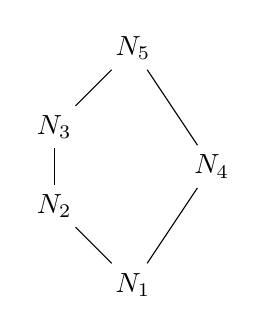
\begin{tikzpicture}

\node (a3) at (7,1) {$N_{1}$};
\node (a4) at (6,2) {$N_{2}$};
\node (a5) at (8,2.5) {$N_{4}$};
\node (a6) at (6,3) {$N_{3}$};
\node (a7) at (7,4) {$N_{5}$};
                  
\draw (a4) -- (a3);
\draw (a5) -- (a3);
\draw (a6) -- (a4);
\draw (a6) -- (a7);
\draw (a5) -- (a7);

\end{tikzpicture}
\caption{Non-distrobutive pentagon Lattice}
\label{fig:p1}
\end{figure}

\begin{lemma}
The function $v$ on this join semilattice $\mathcal{L}$ is a strictly increasing join semi-valuation.
\end{lemma}
\begin{proof} 
Since $\mathcal{L}$ is a lattice, we proof this lemma based on Proposition 5. It is easy to find this function is increasing that $v(N_{1})$$<$$v(N_{2})$$<$$v(N_{3}$$<$$v(N_{4})$$<$$v(N_{5})$. Then we show it satisfies join-modularity: $$\forall x,z\in L, v(x \, \sqcup \,  z) + v(x \, \sqcap \,  z) \leq v(x) + v(z).$$ We only need to check the situation when $x$ represent $N_{4}$ and $z$ represent $N_{2}$ or $N_{3}$, otherwise those two points would be related in this lattice and the modularity law must be satisfied.
\end{proof} 

\begin{lemma}
This join semilattice $\mathcal{L}$ is not (upper) semimodular.
\end{lemma}

\begin{proof} 
We choose $N_{4}$, $N_{2}$ and $N_{1}$ in $\mathcal{L}$ to check. Since we have $N_{4}$$\succ$$N_{1}$ and $N_{1}$$\vee$$N_{2}$=$N_{2}$ and $N_{4}$$\vee$$N_{2}$=$N_{5}$. We find that $N_{2}$$\nprec$$N_{5}$, then we get $N_{1}$$\vee$$N_{2}$$\nprec$$N_{4}$$\vee$$N_{2}$ which do not satisfy the semi-modular law.
\end{proof} 






\section{Semivaluation on Semi-modular lattice}

\subsection{Height function on Semimodular Semilattice}
Before we can describe our result for semivaluation on semilattice,  We first need to introduce the correspondence between height function and semivaluation on semimodular semilattice 

\begin{theorem} Let L be a join semilattice and having a minimum. The following are equivalent: \\

1) L is upper semimodular \\

2) The height function $h$ is a semivaluation. 

\end{theorem}

\begin{proof}
From(i)to(ii): First, we consider the case when x$<$y and z$<$y. Thus we have h(x$\vee$z)$<$h(x$\vee$y). Obviously, we have h(y)$=$h(y$\vee$z). So we get the result: h(x$\vee$z)+h(y)$<$h(x$\vee$y)+h(y$\vee$z).\\\\
Then we consider the more general case when x$>$y or z$>$y. It suffices to verify it when x$>$y, then we have h(x$\vee$y)=h(x). As $\mathcal{L}$ is upper semimodular, based on Gratzer's theorem 375 [Gra11], It is trivially the same for semilattice\footnote{Gratzer verified it using only the single operation which is exactly what we have for semilattice.} that given $C$ to a maximal chain in [y,x], then $D$=\{c$\vee$z $|$ c$\in$C\} is a maximal chain in [y$\vee$z,x$\vee$z]. By the Jordan-Holder Chain Condition, the length of $C$ is h(x)-h(y) which equal to h(x$\vee$y)-h(y). Then the length of $D$ is at most the length of $C$, which is h(x$\vee$z)-h(y$\vee$z). So we get the result: h(x$\vee$z)-h(y$\vee$z)$<$h(x$\vee$y)-h(y).\\\\
For the case when y is no related with x and z, we can verify it by assuming h(y)$>$h(x) or h(y)$<$h(x), respectively. So the processes will be the same as when y$>$x or y$<$x as what we do above.\\\\
From(ii)to(i): Say we have that the height function $h$ is a join semivaluation, then we get  h(x$\vee$z)$\leq$h(x$\vee$y)+h(y$\vee$z)-h(y) by definition which is the same as h(x$\vee$z)-h(y$\vee$z)$\leq$h(x$\vee$y)-h(y). Suppose x$\succ$y, so h(x)=h(y)+1. Then, we can say h(x$\vee$y)=h(y)+1 (as $h$ is the height function). Then it is clearly that h(x$\vee$z)-h(y$\vee$z)$\leq$h(x$\vee$y)-h(y)=1 which means h(x$\vee$z)=h(y$\vee$z)+1 and lead to the result that x$\vee$z $\succ$ y$\vee$z.

\end{proof} 


\subsection{Von Neumann Independence on Semimodular Semilattice}

\begin{definition}
Let $\mathcal{L}$ be a semimodular semilattice satisfying DCC having a minimum. A subset $\mathcal{I}_{n}$ = \{ $a_{1}$, ... ,$a_{n}$\} is called $independent^{*}$ if $$\forall i \in n, \{ \bigvee \mathcal{I}_{i-1}, a_{i} \}\ is\ a\ antichain.$$

%\nexists a_{i} \in \mathcal{I}_{i}, \bigvee \mathcal{I}_{i-1} > a_{i}\ (or\ we\ say:  \forall i \in n, \bigvee \mathcal{I}_{i-1}\ is\ no\ related\ with\ a_{i}) $$.
\end{definition}

\begin{theorem}
Let $\mathcal{I}_{n}$ = \{$a_{1}$, ... ,$a_{n}$\} be an $independent^{*}$ set of a semimodular semilattice with a minimum composed by atoms. Then there is:$$ h(\bigvee \mathcal{I}_{n})=n. $$
\end{theorem}

\begin{proof}
We proof the equation by induction. Given an index $i$, we proof that: $$ h(\bigvee \mathcal{I}_{i}) = i. $$ Obviously, this is true for $i$=1 as $a_{i}$ is an atom. If $h$($\bigvee$$\mathcal{I}_{n}$) = $i$, consider the semimodular law for the height function on $\bigvee$$\mathcal{I}_{i}$ and $a_{i+1}$. Then we obtain: $$ h(\bigvee \mathcal{I}_{i} \vee a_{i+1}) \leq h(\bigvee \mathcal{I}_{i} \vee \bot) + h(\bot \vee a_{i+1}) - h(\bot)$$ As $a_{i+1}$ is also an atom and $\bot$ is the minimum, we obtain h($a_{i+1}$)=1, h($\bot$)=0. Follow this:$$ h(\bigvee \mathcal{I}_{i+1}) \leq h(\bigvee \mathcal{I}_{i}) + 1$$In the same time, consider $\mathcal{I}$ is an $independent^{*}$ set composed all by atoms, trivially we can say that $\bigvee$$\mathcal{I}_{i}$ is no related with $a_{i+1}$ and then $\bigvee$$\mathcal{I}_{i}$ $<$ $\bigvee$$\mathcal{I}_{i+1}$. Based on the condition that height function is strictly increasing which means h($\bigvee$$\mathcal{I}_{i}$) $<$ h($\bigvee$$\mathcal{I}_{i+1}$), so we obtain: $$ h(\bigvee \mathcal{I}_{i+1}) = h(\bigvee \mathcal{I}_{i}) + 1 = i + 1.$$
\end{proof}

\subsection{M-symmetric on Semimodular Semilattice}

\begin{definition}
Let $\mathcal{L}$ be a join semilattice. The pair of elements (a,b) of $\mathcal{L}$ is modular, in notation, a$M^{*}$b: $$\forall x \leq b, if\ \exists y \leq a\ and\ y \leq b, and\ the\ map\ \mathcal{P}:\ [x \vee y, b] \rightarrow [x \vee a, a \vee b]\ is\ one\ to\ one$$ We say the triple \{a,b,y\} is a modular triple and the semilattice $\mathcal{L}$ is called M-symmetric if a$M^{*}$b implies that b$M^{*}$a for every a,b$\in$ $\mathcal{L}$ .
\end{definition}

\begin{corollary}
$\forall$ x $\leq$ b, if $\exists$ y $\leq$ a and y $\leq$ b and a$M^{*}$b in semilattice $\mathcal{L}$, then we obtain the following equivalence for the height function of  $\mathcal{L}$:\\

1) h(a$\vee$b) - h(x$\vee$a) = h(b) - h(x$\vee$y)\\

2) h(a$\vee$b) = h(a$\vee$y) + h(y$\vee$b) - h(y)\\

The equation 2) lead to a result that the join valuation (see the equivalence in Corollary 17) on the modular tripe \{a,b,y\} is also a join co-valuation. Then we can say that the constraint for modular pair is more strict than the law for semivaluation.  

\end{corollary}

\begin{proof}
1): Note that by definition 18, we obtain the map $\mathcal{P}$: [x $\vee$ y, b] $\rightarrow$ [x $\vee$ a, a $\vee$ b] is one to one which indicate that the length of this two internals linked by map $\mathcal{P}$ is equivalent. In another word, the maximal chains for each of them have the same length which lead to our equation on height function.

2):  Consider 1), we can use $y$ to replace $x$ in the equation. Based on the condition, we also have  h(y$\vee$b)=h(b). Thus, we obtain the equation 2).

\end{proof}

\begin{theorem}
Let $\mathcal{L}$ be a join semilattice. $\mathcal{L}$ is semimodular if it is M-symmetric.
\end{theorem}
\begin{proof}
 Let a,b,c $\in$ $\mathcal{L}$ and let b $\succ$ a. Obviously, We have  b$\vee$c$ \geq $a$\vee$c. When b$\vee$c = a$\vee$c, it leads to the result that  b$\vee$c $\succ$ a$\vee$c directly. So we proof the case when b$\vee$c $>$ a$\vee$c below.
 
Put d=a$\vee$c, then we need to prove b$\vee$c $\succ$ d. Let x that b$\vee$c $\succ$ x and x $\geq$ d. Then we find there is a one to one map from [a, b]to[x, b$\vee$c]. So for all z $<$ b, it follows that the map $\mathcal{P}_{1}$:[z$\vee$a, b]$\rightarrow$[z$\vee$x, x$\vee$b] is one to one, then we obtain that x$M^{*}$b.
 
By M-symmetry, we obtain  b$M^{*}$x simultaneously, which means, by definition, the map $\mathcal{P}_{2}$: [d$\vee$a, x] $\rightarrow$ [d$\vee$b, b$\vee$x] is one to one (based on the condition that x $\geq$ d and b $>$ a, so c $<$ x and a $<$ x,b). Consider we have b$\vee$c $\succ$ x and b$\vee$c $>$ d, then it suffices to say that b$\vee$c = b$\vee$x = d$\vee$b which means the right side of $\mathcal{P}_{2}$ contains only one node. This lead to that the left side of $\mathcal{P}_{2}$ can only contains one node as well. So we obtain the result that x = d$\vee$a = d. Finally, We get  b$\vee$c $\succ$ a$\vee$c.
 
We give the \textbf{Figure \ref{fig:sit}} for easier understanding. A similar result and graph for lattice has given on Gratzer's Theorem 384 and Theorem 385 [Gra11].

\end{proof}

\noindent{\bf Note:} We do not obtain a trivial injection in Theorem19. We find that a semilattice may not contains any modular pairs when it does not have a $\bot$ ( or we say a $strictly$ semilattice ) because there may not be such a $y$ as in definition19 in general. 

Consider a basic semilattice $\mathcal{L}_{3}$ = \{N1,N2,N3\} in which N1 $\succ$ N2 and N1 $\succ$ N3, respectively. It is obvious that no pairs $\mathcal{L}_{3}$ have a meet, then we can say it doesn't contain any modular pairs and it can not be M-symmetric. 

\begin{figure}
\center
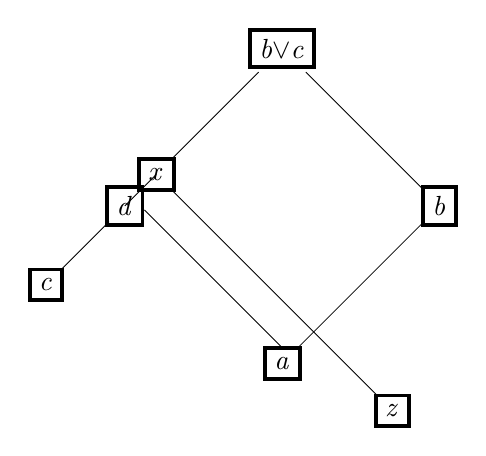
\begin{tikzpicture}
\node[draw,line width=0.5mm] at (4,6) {\textit{b$\vee$c}};
\node[draw,line width=0.5mm] at (2.4,4.4) {\textit{x}};
\node[draw,line width=0.5mm] at (2,4) {\textit{d}};
\node[draw,line width=0.5mm] at (6,4) {\textit{b}};
%\node[draw] at (4.2,2.2) {\textit{z$\vee$a}};
\node[draw,line width=0.5mm] at (4,2) {\textit{a}};
\node[draw,line width=0.5mm] at (5.4,1.4) {\textit{z}};
\node[draw,line width=0.5mm] at (1,3) {\textit{c}};

 \draw[-,line width=0.1mm] (3.7,5.7) -- (2.6,4.6);
 \draw[-,line width=0.1mm] (2.4,4.4) -- (2,4);
  \draw[-,line width=0.1mm] (2.25,3.95) -- (4,2.2);
  \draw[-,line width=0.1mm] (2.6,4.2) -- (4.4,2.4);
  \draw[-,line width=0.1mm] (4.2,2.2) -- (4.4,2.4);
  \draw[-,line width=0.1mm] (4.4,2.4) -- (5.8,3.8);
  \draw[-,line width=0.1mm] (5.8,4.2) -- (4.3,5.7);
  \draw[-,line width=0.1mm] (4.4,2.4) -- (5.2,1.6);
  \draw[-,line width=0.1mm] (1.8,3.8) -- (1.2,3.2);
     
\end{tikzpicture}
\caption{Modular elements on semilattice} 
\label{fig:sit}
\end{figure}

\section{Semivaluation and Order Dimension}
In this section, we first recall the notation, Order Dimension and Realizer [Dus41] on a poset. The connection between Order Dimension theory and Valuation on modular (distributed) lattice through Birkhoff's representation theorem [Bir84] has been indicated by Marigo [Mar12]. Then, We maintain the bottleneck of extending this theorem on semi-modular lattice and non-modular lattice based on the fact that we can not view those kind of lattices as downsets of poset. \\\\While by considering the order dimension on semi-modular lattice directly, we can generate a novel approach to build up the Semivaulation on semimodular lattice by realizer which shown in Theorem 18.

\subsection{Order Dimension and Realizer}
\begin{definition}
(Dushink, Ben; Miller, E. W.) Given a poset $\mathcal{P}$, we define the order dimension of $\mathcal{P}$ $\leq$ $n$ iff there is a set $R$ of linear extensions of $\mathcal{P}$:  $R$ = \{ $\bigwedge_{1}$,$\bigwedge_{2}$,..., $\bigwedge_{n}$\} such that:\\

1) $\forall$x,y $\in$ $P$, if x $\leq$ y in $P$, then $\forall$$\bigwedge_{i}$$\in$$R$, x $\leq$ y in $\bigwedge_{i}$ \\

2) $\forall$x,y $\in$ $P$, if x $\nleq$ y in $P$, then $\exists$$\bigwedge_{i}$$\in$$R$, y $\leq$ x in $\bigwedge_{i}$\\

We name $R$ the realizer of $\mathcal{P}$, the order dimension is $n$ iff $n$ is the least number of linear extensions in $R$. 

\end{definition}

\begin{theorem}
(Marigo) There is a bijection between finite distributed lattice with complete valuations and poset whose order dimension is no more than two. 
\end{theorem}

\subsection{Generate Semivaluation from Realizer on modular lattice}

We can use a similar way based on the theorem above as indicated by Marigo [Mar12] to generate a semivaluation from realiser through the Birkhoff's representation theorem on modular lattice.\\\\
Given a modular lattice $\mathcal{L}$, view it as composed by downsets by inclusion of a corresponding poset $\mathcal{P}$ whose order dimension is no more than two, with a realiser $R$:\{$\bigwedge_{1}$,$\bigwedge_{2}$\}, we first inverse the order in $\bigwedge_{2}$ to create a complementary realiser $R'$: \{$\bigwedge_{1}$,$\bigwedge'_{2}$\} which indicate a complementary poset of $\mathcal{P}$. \\\\
Then we use the weight function $\omega$(x) on this complementary poset which counting chains from each node. After this, we can define the semivaluation (which is actually as valuation) on $\mathcal{L}$ as below: $$ \forall a \in \mathcal{L}, v(a)=\sum_{x \in a_{\downarrow}} \omega(x)  $$ We refer to [Mar12] for the proof of the correctness of this process as it is the similar way indicated in there.

\subsection{Bottleneck of Birkhoff representation on semimodular and non-modular lattice}
\subsubsection{On semimodular lattice}
Consider the typical semimodular lattice below, 
\subsubsection{On non-modular lattice}

\subsection{Generate Semivaluation from Realizer on semimodular semilattice}
Instead of viewing the semimodular semilattice as downsets of a poset, we consider the realiser of the semilattice as a constraint poset and build up the semivaluation on this semilattice directly. Before describe the Semivaluation, first we need define the height function on linear extension and realiser.

\begin{definition}
Given a poset $\mathcal{P}$, we define the height function h on a linear extension $L$ of  $\mathcal{P}$ as follow:\\

1) $\forall$$x_{i}$$\in$ $L$,  if $x_{0}$$\leq$$x_{i}$, $h_{l}$($x_{0}$) = 1\\

2) $\forall$$x_{i}$,$x_{j}$$\in$ $L$, if $x_{i}$$\succ$$x_{j}$, $h_{l}$($x_{i}$)=$h_{l}$($x_{j}$)+1  

\end{definition}

\begin{definition}
Given a poset $\mathcal{P}$, we define the Total height function H on a realiser $R$ of $\mathcal{P}$ as follow:\\ 

$H_{R}(x)$ = $\sum_{l\in R}$$h_{l}$(x)

\end{definition}

\noindent{\bf Note:} We loosely refer $H_{R}(x)$ on poset $\mathcal{P}$ with realiser $R$ as $H(x)$ based on the trivial symmetry on different realisers for a certain poset.\\\\

Now we can generate the semivaluation directly from the realiser on semilattice which indicated by the following theorem.

\begin{theorem}
Total height function H(x) on a semimodular semilattice $L$ is a semivaluation.
\end{theorem}

\begin{proof}

Given a semimodular semilattice $L$ with realiser $R$, We proof it by induction on the value $n$ of order dimension ( the number of linear extensions in $R$). 

We first consider the case when n=1 which means $L$ is an linear order. Then trivially we obtain $H(x)$=$h(x)$ and the height function on the linear extension is actual the height function on the lattice, based on Theorem 11 above, the result is easily shown. 

Then we suppose the result has been proved when n=k-1: $$ H(x \, \sqcup \,  z) \leq H(x \, \sqcup \,  y) + H(y \, \sqcup \, 
 z) -H(y) $$ we want to present it also satisfy the law when n=k which means $$ H(x \, \sqcup \,  z)+h_{k}(x \, \sqcup \,  z) \leq H(x \, \sqcup \,  y) +h_{k}(x \, \sqcup \,  y) + H(y \, \sqcup \, z)+h_{k}(y \, \sqcup \,  z)  -(H(y)+h_{k}(y) ) $$ then we only need to proof: $$ h_{k}(x \, \sqcup \,  z) \leq h_{k}(x \, \sqcup \,  y) + h_{k}(y \, \sqcup \,  z)  - h_{k}(y)  $$ Due to the fact that $k$ is a new linear extension belong to R, so x, y must be comparable in $k$. Based on the symmetry on the notation of semivaulation, we only need to proof one case such as x $>$ z. Then $h_{k}$(x\, $\sqcup$\,  z)= $h_{k}$(x). Consider $h_{k}$(x)$\leq$$h_{k}$(x\, $\sqcup$\,  y) and $h_{k}$(y)$\leq$$h_{k}$(y\, $\sqcup$\,  z), we verified the result.

\end{proof}


\begin{thebibliography}{fi99}

\bibitem[Bir84] {bi} G. Birkhoff, {\it Lattice Theory}, AMS Colloquium Publications {\bf 25}, Providence, Rhode Island, 1984. 

\bibitem[Dus41] {bi} Dushink, Ben; Miller, E. W. {\it Partially ordered sets}, American Journal of Mathematics, 1941.

\bibitem[Gra11] {gi} G.Gratzer, {\it Lattice Theory:Foundation}, 
Springer Basel, 14 Feb 2011.

\bibitem[Mar12] {bi} Francesco Marigo, {\it Complete Valuations on Finite Distributive Lattices}. 24 Nov, 2012.

\bibitem[Sch97] {ms2} M. P. Schellekens, Complexity Spaces: Lifting \& Directedness, {\it Topology Proceedings} {\bf 22}, 403 - 425, 1999. 

\bibitem[Sch04] {semival} M.P. Schellekens, The correspondence between partial metrics and semivaluations, {\it Theoretical Computer Science}, Volume 315, Issue 1, 5 May 2004, 135–149, 2004. 

\bibitem[Sch03] {qd} M. P. Schellekens, A characterization of partial metrizability:
domains are quantifiable,  {\it Theoretical Computer Science}, Volume 305, 409 - 432, 2003. 

\bibitem[SYRV14] {syrv} M. Schellekens, T. Yu, S. Romaguera, O. Valero, {\it On Semivaluations and Semimodularity} (preprint, 2014, submitted to journal Order).

\end{thebibliography}

\end{document}



%--------------------------
%below is a unsuccessful correspondence
%-------------------------

We come up with a conjecture that there may be a correspondence between Semimodular lattices and Finite Partial Order set of dimension at most two.  First, we use the idea based on $Birkhoff's$ $representation$ $theorem$[Bir84] applying on non-distributive lattice. We proof that as for a typical partial order set with dimension[Dus41] more than two (containing $\mathcal{N}$ shape), the corresponding lattice of downsets of it must contain a pentagon sublattice which is a typical non-distributive lattice. Then, we proof this pentagon sublattice is not only non-distributive, but also non-semimodular by a counter example. Then, we infer that a semimodular lattice's corresponding poset cannot contain a $\mathcal{N}$ shape, so its order dimension is at most two. We have not found the corresponding pairs of linear extensions to proof the bijection but it may be done like [Mar12].

\subsection{Poset and Non-Semimodular Lattice}
Consider a typical poset with dimension more than two, as shown in \textbf{Figure \ref{fig:p1}}. We label each node in this $\mathcal{N}$ shape as shown in the figure. Then based on the idea from $Birkhoff's$ $representation$ $theorem$, we use the downsets of this poset with the unions and intersections operation to constract a corresponding lattice, also shown in \textbf{Figure \ref{fig:p1}}.
\subsection*{Theorem 1} 
A poset of $\mathcal{N}$ shape corresponding lattice (by downsets) must contain a pentagon sublattice.\\\\
Proof:\\\\
{\it Consider the node C in \textbf{Figure \ref{fig:p1}}. C$\succ$B and D$\succ$B and C is no relation with D, then the downsets composed by those three nodes are: CDB, CB, DB, B. It is easy to say that they construct a quadrilateral lattice, which contains two chains: CDB$\succ$DB$\succ$B and CDB$\succ$CB$\succ$ B.\\\\ 
Then, as a $\mathcal{N}$ shape, there must exist a node A which is covered by C or D and no relation with other nodes in this poset. We assume C$\succ$A, as in \textbf{Figure \ref{fig:p1}}. Then we get two new downsets BA and A whilst update the downsets CDB and CB to CDBA and CBA, respectively. \\\\Then we find that the new coming node BA must be inserted between CBA and B in the corresponding lattice and neither BA or CBA is still no relation with DB which make the old quadrilateral lattice to be a pentagon sublattice in the updated lattice,as shown in \textbf{Figure \ref{fig:p2}}.}

\subsection*{Theorem 2}
Pentagon sublattice is non-semimodular\\\\
Proof:\\\\
{\it Consider this non-distributive sublattice $\mathcal{L}$, as shown in \textbf{Figure \ref{fig:p2}}. As labelled in this figure, we can find that x$\wedge$y$\prec$y but x$\nprec$x$\vee$y. Then we get, in this lattice, x$\wedge$y$\prec$y$\nRightarrow$x$\prec$x$\vee$y. So we say pentagon sublattice is non-semimodular.}



\begin{figure}
\centering
\begin{tikzpicture}
  \node (a2) at (2,1) {$A$};
 \node (a3) at (3,1) {$B$};
  \node (a4) at (2,2) {$C$};
   \node (a5) at (3,2) {$D$};
 \draw (a4) -- (a3);
 \draw (a4) -- (a2);
 \draw (a5) -- (a3);
   \node (a1) at (6,0) {$-$};
 \node (a2) at (5,1) {$A$};
 \node (a3) at (7,1) {$B$};
  \node (a4) at (6,2) {$AB$};
   \node (a5) at (8,2.5) {$BD$};
    \node (a6) at (6,3) {$ABC$};
       \node (a7) at (7,4) {$ABCD$};
 \draw (a1) -- (a3);
 \draw (a1) -- (a2);
 \draw (a4) -- (a2);
 \draw (a4) -- (a3);
 \draw (a5) -- (a3);
\draw (a6) -- (a4);
\draw (a6) -- (a7);
\draw (a5) -- (a7);

 
\end{tikzpicture}
\caption{Poset with $\mathcal{N}$ shape and corresponding Lattice by downsets}
\label{fig:p1}
\end{figure}

\begin{figure}
\centering
\begin{tikzpicture}

 \node (a3) at (7,1) {x$\wedge$y};
  \node (a4) at (6,2) {$x$};
   \node (a5) at (8,2.5) {$y$};
    \node (a6) at (6,3) {$z$};
       \node (a7) at (7,4) {x$\vee$y};
                  
 \draw (a4) -- (a3);
 \draw (a5) -- (a3);
\draw (a6) -- (a4);
\draw (a6) -- (a7);
\draw (a5) -- (a7);

 
\end{tikzpicture}
\caption{Non-distrobutive pentagon Lattice}
\label{fig:p2}
\end{figure}

\subsection{Poset and Semimodular Lattice}
Based on $Birkhoff's$ $representation$ $theorem$, there exist a one-to-one correspondence between distributive lattices and partial orders. Then there exist a correspondence between semimodular lattice and partial order in the same way as all distributive lattice is modular. We have proven that in this way, a non-semimodular lattice's corresponding poset must contain a $\mathcal{N}$ shape which means its order dimension must more than three. So we infer that a semimodular lattice cannot have a corresponding poset which contain $\mathcal{N}$ shape and order dimension more than three. So we come up with a conjecture below:
\subsection*{Conjecture 1}
{\it There exist a bijection between Semimodular lattice and Partial Order Set with dimension at most two.}\\\\

It is hard to find the corresponding pairs of linear extensions to proof the conjecture. One way to build them is like in [Mar12] when we consider the valuation, or say semivaluation for semimodular lattice. The problem is that we can only using the single operation when focus on semivaluation, so we cannot use the duality to find a 'diametral' linear extension.
